\section{結果}
\subsection{ストレッチセンサ計測精度評価}
Fig. \ref{output_for_test}のような出力を各空気圧人工筋に与えた結果,
Table.\ref{strain}のような長さの結果となった.
また,それぞれの時におけるストレッチセンサ時定数の結果を求めると,Table.\ref{4_2}に示す様になった.
\begin{table}[h]
    \caption{ストレッチセンサ 長さ(mm) 計測結果}
    \label{strain}
    \begin{center}
        \begin{tabular}{|c|c|ccc|}\hline
            \multicolumn{2}{|c|}{} & \multicolumn{3}{c|}{筋肉種類}\\
            \cline{3-5}
            \multicolumn{2}{|c|}{} & 前脛骨筋 & 腓骨筋 & ヒラメ筋 \\ \hline
            & 1 & 236 & 194 & 208 \\ \cline{2-5}
            & 2 & 234 & 197 & 210 \\ \cline{2-5}
            & 3 & 233 & 198 & 213 \\ \cline{2-5}
            & 4 & 234 & 199 & 214 \\ \cline{2-5}
            & 5 & 220 & 204 & 215 \\ \cline{2-5}
            計測位置 & 6 & 208 & 217 & 225 \\ \cline{2-5}
            & 7 & 214 & 217 & 227 \\ \cline{2-5}
            & 8 & 215 & 215 & 223 \\ \cline{2-5}
            & 9 & 218 & 203 & 218 \\ \cline{2-5}
            & 10 & 233 & 195 & 216 \\ \cline{2-5}
            & 11 & 234 & 192 & 212 \\ \cline{2-5}
            & 12 & 235 & 197 & 209 \\ \hline
        \end{tabular}
    \end{center}
\end{table}

\newpage

%セルを結合して中央揃え
%(参考):https://qiita.com/ta_b0_/items/c8c828b6a53d49498736
\begin{table}[h]
    \caption{ストレッチセンサ 時定数(us) 計測結果}
    \label{4_2}
        \begin{center}
            \begin{tabular}{|c|c|ccc|}\hline
            \multicolumn{2}{|c|}{} & \multicolumn{3}{c|}{筋肉種類}\\
            \cline{3-5}
            \multicolumn{2}{|c|}{} & 前脛骨筋 & 腓骨筋 & ヒラメ筋 \\ \hline
            & 1 & 43.86±0.02 & 68.14±0.03 & 40.13±0.01 \\ \cline{2-5}
            & 2 & 44.42±0.02 & 68.07±0.02 & 40.13±0.01 \\ \cline{2-5}
            & 3 & 44.73±0.02 & 68.07±0.02 & 39.26±0.01 \\ \cline{2-5}
            & 4 & 44.50±0.01 & 67.12±0.04 & 38.43±0.02 \\ \cline{2-5}
            & 5 & 46.74±0.01 & 66.86±0.02 & 38.45±0.01 \\ \cline{2-5}
            計測位置 & 6 & 46.93±0.02 & 63.37±0.01 & 37.24±0.01 \\ \cline{2-5}
            & 7 & 47.03±0.01 & 64.74±0.05 & 37.33±0.01 \\ \cline{2-5}
            & 8 & 47.02±0.01 & 64.76±0.03 & 37.17±0.01 \\ \cline{2-5}
            & 9 & 46.80±0.01 & 65.92±0.03 & 37.38±0.01 \\ \cline{2-5}
            & 10 & 44.20±0.01 & 66.76±0.04 & 38.21±0.01 \\ \cline{2-5}
            & 11 & 44.74±0.01 & 66.92±0.05 & 38.46±0.01 \\ \cline{2-5}
            & 12 & 45.13±0.02 & 66.90±0.03 & 38.65±0.01 \\ \hline
        \end{tabular}
    \end{center}
\end{table}

\subsection{ストレッチセンサ動的計測}

Fig. \ref{output_for_actions}のような出力を各空気圧人工筋に与え,
1秒ごとに区切り0.01秒ごとの区間の平均値,標準誤差の計算を行った結果,
Fig.\ref{zenkei_action},\ref{hikotsu_action},\ref{hirame_action}に示すようになった.
\begin{figure}[h]
  \begin{center}
  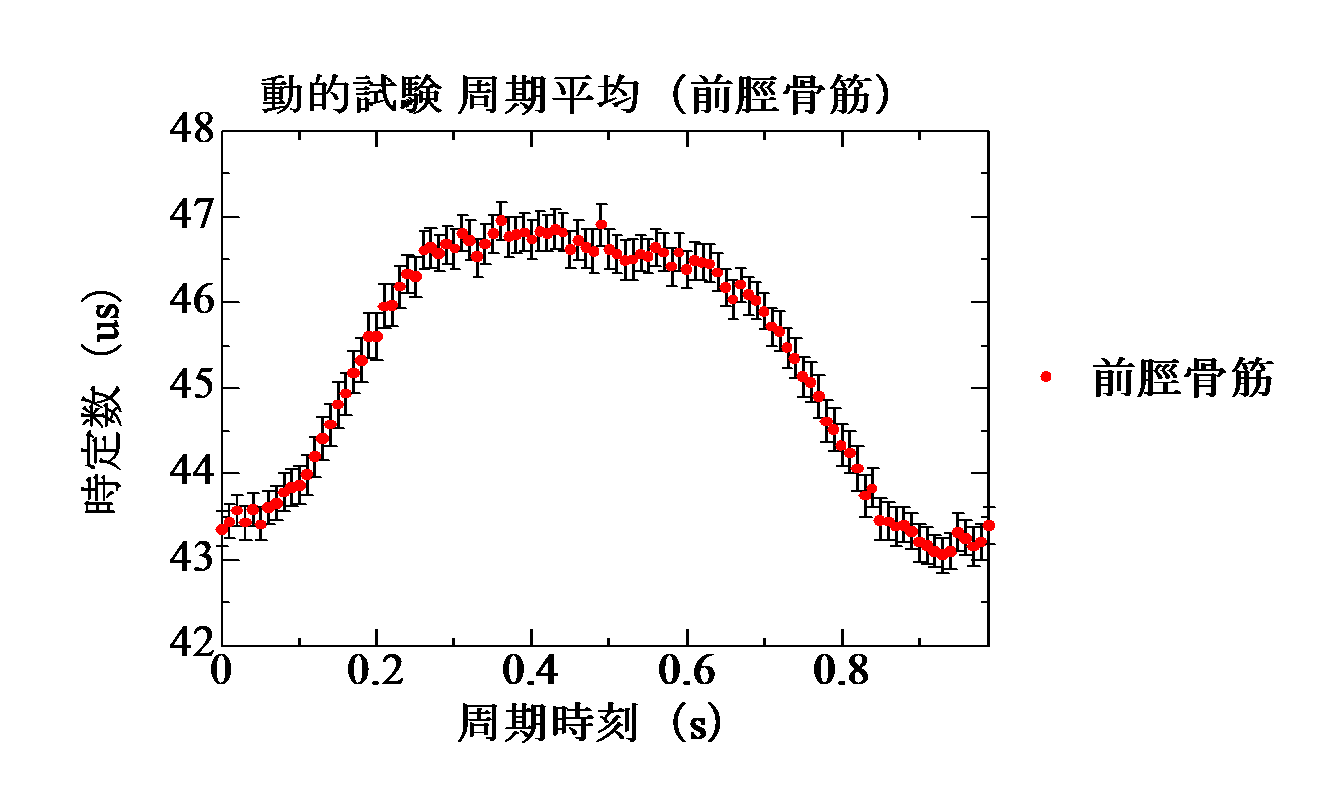
\includegraphics[width=0.75\columnwidth,clip]{./4_consideration/moving/zenkei.eps}
  \caption{ストレッチセンサ動的計測結果(前脛骨筋)}
  \label{zenkei_action}
  \end{center}
\end{figure}
\begin{figure}[h]
  \begin{center}
  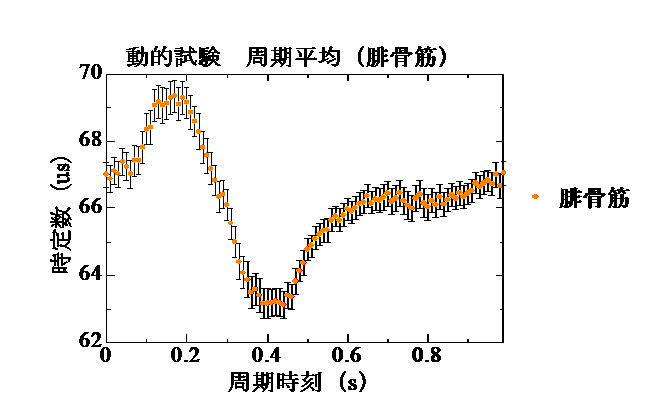
\includegraphics[width=0.75\columnwidth,clip]{./4_consideration/moving/hikotsu.eps}
  \caption{ストレッチセンサ動的計測結果(腓骨筋)}
  \label{hikotsu_action}
  \end{center}
\end{figure}

\clearpage

\begin{figure}[h]
  \begin{center}
  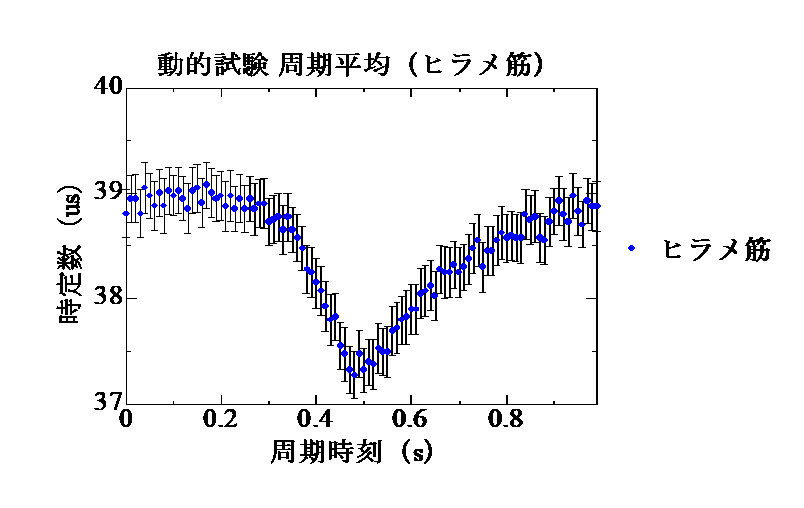
\includegraphics[width=0.75\columnwidth,clip]{./4_consideration/moving/hirame.eps}
  \caption{ストレッチセンサ動的計測結果(ヒラメ筋)}
  \label{hirame_action}
  \end{center}
\end{figure}

\section{考察}
\subsection{ストレッチセンサ計測精度}
先ほどの結果より,それぞれの計測位置における空気圧人工筋の長さをグラフに表すと,
Fig.\ref{4-ml}の様になった.このグラフから見てわかるように,腓骨筋とヒラメ筋が組となって
前脛骨筋と逆位相のsin波形的動きをさせることが出来た.今回,足関節ロボットの空気圧人工筋
それぞれに対して,Fig.\ref{output_for_test}の出力を出すよう指令を与えたので
システムとして問題なく動いたことがわかった.

続いて,Table.\ref{4_2}の結果を用いて,横軸にセンサの長さ,縦軸に時定数としたグラフを
描画すると,Fig.\ref{ml-rc1},\ref{ml-rc2},\ref{ml-rc3}に示すようになった.
各筋肉に関して,長さが増加するとセンサでの計測値が減少した.
どの筋肉においても同様の結果を示しており,ストレッチセンサが伸びると
静電容量が減少するといったことが分かった.

一方でセンサごとに空気圧人工筋の長さに対する計測値の変化の特性が異なる.これは,
センサ自体が自作されており,その製作時のむらによるものだと考えられる.それに加えて,
空気圧人工筋に設置する時にある程度テンションを与えて設置するのだが,そのテンションの
かけ方具合にもよると考えられる.実際に使用するときは,ストレッチセンサを空気圧人工筋に
設置した状態で,今回の実験の様にセンサ特性の解析を行う必要があると考えられる.

また,空気圧人工筋の伸びの変化に対して,時定数の変化が非常に微小なものとなっている.
今回の時定数の結果や,製作したRC回路の抵抗値$1.5M\Omega$より静電容量の変化量に関して考えると,
最も変化が大きかった腓骨筋においても$42~45pF$の変化しか現れなかった.
これに対する対策として,RC回路における抵抗値の再選定を行う必要があると考えられた.
抵抗値を増加させると時定数も増加するのでマイコンで変化量を計測しやすくなる.
一方で,抵抗値を増大させると計測ノイズ成分も大きくなるので,その辺りも踏まえて抵抗値の
再選定をしていく必要があると考えられる.

\begin{figure}[h]
    \begin{center}
        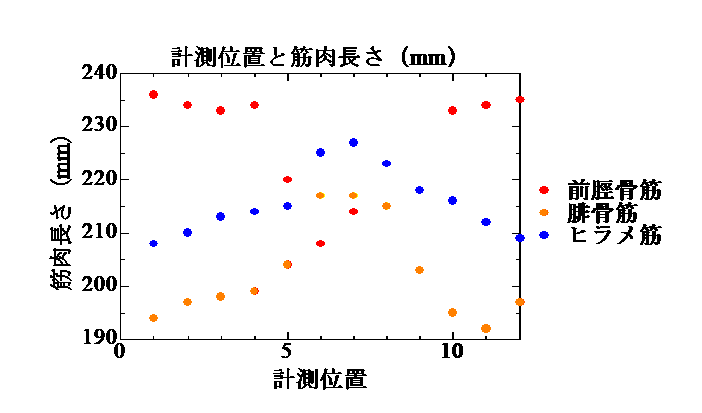
\includegraphics[width=0.7\columnwidth,clip]{4_consideration/ml.eps}
    \end{center}
    \caption{計測位置と各空気圧人工筋の長さの関係}
    \label{4-ml}
\end{figure}

\begin{figure}[h]
    \begin{center}
        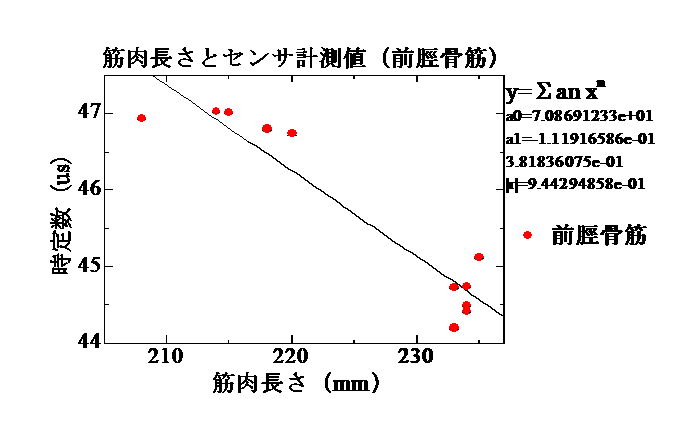
\includegraphics[width=0.7\columnwidth,clip]{4_consideration/zenkei.eps}
    \end{center}
    \caption{空気圧人工筋の長さとセンサ計測値の関係(前脛骨筋)}
    \label{ml-rc1}
\end{figure}
\clearpage
\begin{figure}[h]
    \begin{center}
        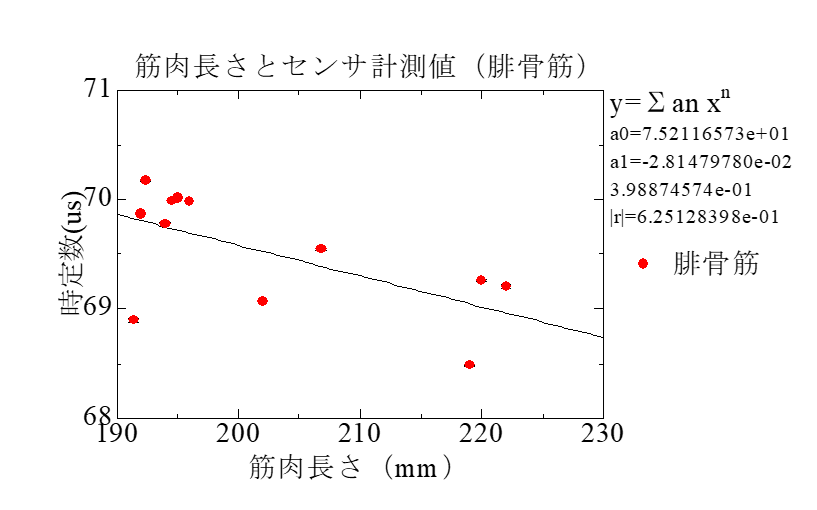
\includegraphics[width=0.7\columnwidth,clip]{4_consideration/hikotsu.eps}
    \end{center}
    \caption{空気圧人工筋の長さとセンサ計測値の関係(腓骨筋)}
    \label{ml-rc2}
\end{figure}
\begin{figure}[h]
    \begin{center}
        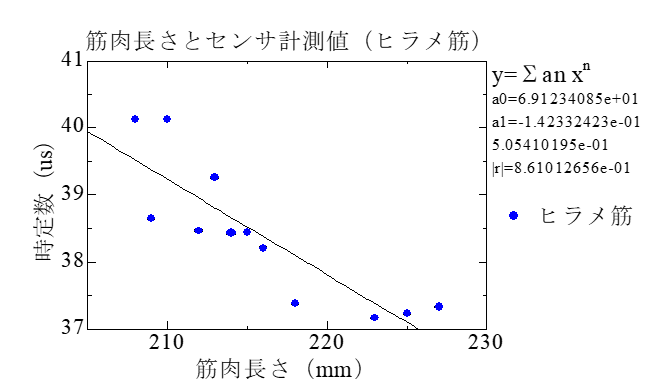
\includegraphics[width=0.7\columnwidth,clip]{4_consideration/hirame.eps}
    \end{center}
    \caption{空気圧人工筋の長さとセンサ計測値の関係(ヒラメ筋)}
    \label{ml-rc3}
\end{figure}
\clearpage
\subsection{ストレッチセンサ動的計測}
今回,各筋肉に1Hzの周期動作を入れ,区間ごとに区切り各平均値の計算を行った.
おおむね,各筋において計測精度評価にて観測された時定数内に収まっていた.これは,
ストレッチセンサを用いた,筋肉の伸縮計測において,再現性があると考えられる.
また,静的にストレッチセンサの実長さの計測を行った上で,ストレッチセンサを用いて
時定数の計測を行うと,実長さが算出できることが分かった.

一方で,今回足関節ロボットの空気圧人工筋動作システムとストレッチセンサの計測システムが,
実装の仕様上,同一システム上となっていないので,足関節ロボットが動作している途中からの
ストレッチセンサの計測となった.このことにより,ストレッチセンサの計測開始と,
空気圧人工筋の出力開始とが合っていない状態となってしまった.
また,計測システムの都合上それぞれのストレッチセンサに対して独立に計測を行ったため,
それぞれのストレッチセンサの計測開始位置も合っていない状態となっている.

上記のことを補正するため,前脛骨筋に関しては時定数の最小値を,腓骨筋,ヒラメ筋に関して最大値を
0秒として処理した.このように処理した理由として,Fig.\ref{output_for_actions}にて示す
出力を各空気圧人工筋に与えたこと,また,Fig.\ref{ml-rc1},\ref{ml-rc2},\ref{ml-rc3}に示す
ように,空気圧人工筋の実長さに対して,時定数は単調減少となってことが元となっている.
これらの結果より,周期位置の補正結果はFig.\ref{min-rc1},\ref{min-rc2},\ref{min-rc3}に示すようになった.
また,それぞれの筋における周期時刻補正後の時定数最小値/最大値の周期時刻は下記の Table.\ref{min-max}に
示すようになった.これらの結果より,背屈方向にかかる時間よりも底屈方向にかかる時間の方が長いことが分かった.
本来であれば,1Hzのsin動作であり,底屈動作,背屈動作ともに0.5sで行われるべき動作である.
これは,重力の影響により,底屈動作よりも背屈動作の方が行われやすかったからと考えられる.
これらの確認として,実際に空気圧人工筋に与えている出力とストレッチセンサの時定数の関係を調べる必要があるとも考えられる.
\begin{table}[h]
  \begin{center}
    \label{min-max}
    \caption{周期時刻補正後の時定数最大値/最小値における周期時刻}
    \begin{tabular}{|c||c|c|c|}\hline
      & 前脛骨筋 & 腓骨筋 & ヒラメ筋 \\ \hline \hline
      最小値 & 0.00s & 0.27s & 0.31s \\ \hline
      最大値 & 0.43s & 0.00s & 0.00s \\ \hline
    \end{tabular}
  \end{center}
\end{table}

\begin{figure}[h]
    \begin{center}
        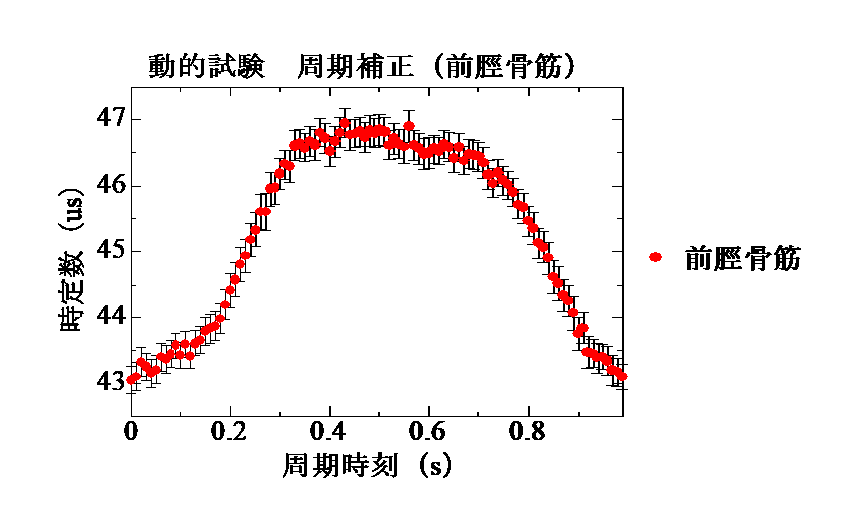
\includegraphics[width=0.75\columnwidth,clip]{4_consideration/min/zenkei.eps}
    \end{center}
    \caption{動的計測 補正結果(前脛骨筋)}
    \label{min-rc1}
    \begin{center}
        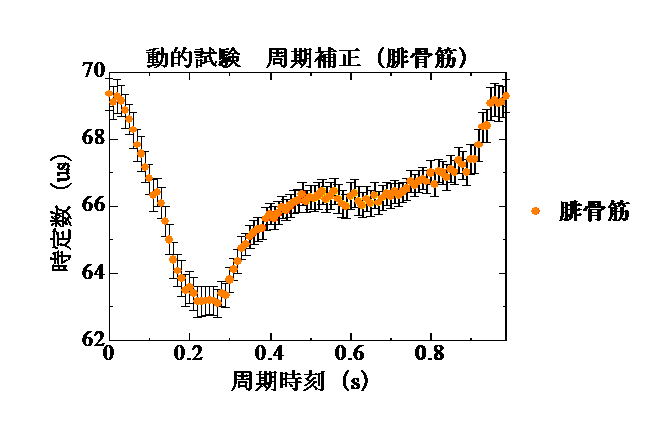
\includegraphics[width=0.75\columnwidth,clip]{4_consideration/min/hikotsu.eps}
    \end{center}
    \caption{動的計測 補正結果(腓骨筋)}
    \label{min-rc2}
\end{figure}
\begin{figure}[t]
    \begin{center}
        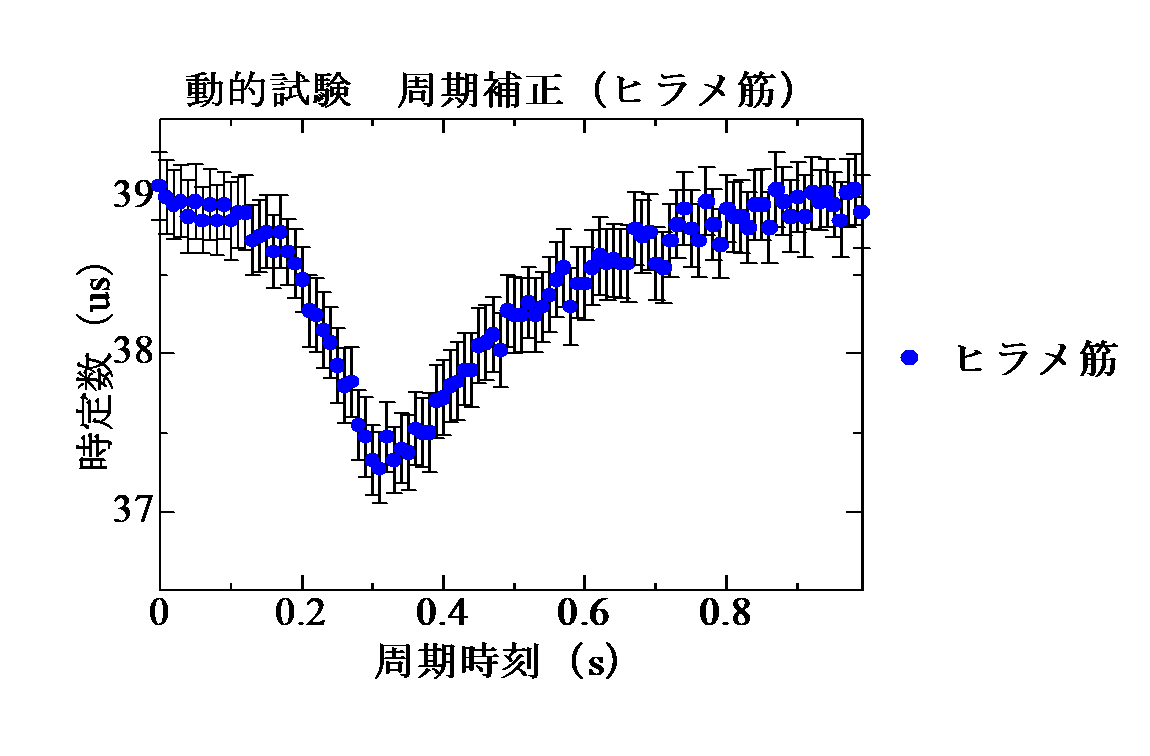
\includegraphics[width=0.75\columnwidth,clip]{4_consideration/min/hirame.eps}
    \end{center}
    \caption{動的計測 補正結果(ヒラメ筋)}
    \label{min-rc3}
\end{figure}
